\documentclass[tikz,border=10pt]{standalone}
\usetikzlibrary{arrows.meta, calc}

\begin{document}
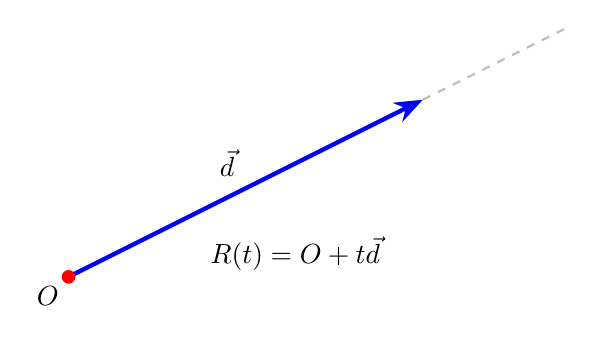
\begin{tikzpicture}[>=Stealth, scale=1.5]

    % Coordinates
    \coordinate (O) at (0,0);      % Origin
    \coordinate (D) at (3,1.5);    % Direction point (end of vector d)
    \coordinate (E) at ($(O)!1.4!(D)$); % Visual "end" of the ray for labeling

    % 1. Draw the infinite extension (dashed)
    \draw[dashed, gray!50, thick] (D) -- (E);

    % 2. Draw the direction vector d
    \draw[->, blue, ultra thick] (O) -- (D) 
        node[midway, above left, black] {$\vec{d}$};

    % 3. Mark the Origin O
    \filldraw[red] (O) circle (1.5pt) 
        node[below left, black] {$O$};

    % 4. Ray Equation placed near the end of the line
    \node[anchor=west, xshift=5pt] at (1, 0.2, 0) {$R(t) = O + t\vec{d}$};

\end{tikzpicture}
\end{document}